\documentclass[12pt,letterpaper,toc=flat,oneside]{report}
\usepackage[top=1in,bottom=1.25in,hmargin=1.25in]{geometry}
\usepackage{textcomp}
\usepackage{setspace}
\usepackage[T1]{fontenc}
\usepackage[utf8]{inputenc}
\DeclareUnicodeCharacter{2122}{!!!!I-AM-HERE!!!!!}
\usepackage[pdftex]{graphicx}
\DeclareGraphicsExtensions{.jpg, .pdf, .png}
\usepackage{color}
\usepackage{xcolor}
\usepackage[linktocpage=true]{hyperref}
\hypersetup{%
    colorlinks,
    linkcolor={red!50!black},
    citecolor={blue!50!black},
    urlcolor={blue!80!black},
    filecolor={blue!80!black},
    urlbordercolor={blue!80!black},
    pdfborderstyle={/S/U/W 1}
}
\usepackage{scripts/tex/acrotex/eforms}
\usepackage{bigstrut, multirow}
\usepackage{ifthen}
\usepackage[scaled=.8]{helvet}
\newenvironment{myfont}{\fontfamily{phv}\selectfont}{\par}
\usepackage[font={bf,normal},labelsep=period,labelfont=bf]{caption}
\usepackage{indentfirst}
\usepackage{float}
\usepackage{flafter}
\usepackage{amssymb,amsmath,amsfonts}
%\usepackage{theorem}  % uncomment if using rmarkdown::pdf_document
\usepackage[numbers,square]{natbib}
\bibliographystyle{abbrvnat}
\usepackage{varioref} 
%\usepackage{tocbibind} 
\usepackage{xspace}
% \usepackage{fixltx2e}
\usepackage{threeparttable}
\usepackage{booktabs}
\usepackage{url}
\usepackage[raggedright]{titlesec}
\usepackage{titletoc}
\usepackage{ifpdf}
\usepackage{lastpage}
\providecommand{\tightlist}{%
\setlength{\itemsep}{0pt}\setlength{\parskip}{0pt}}
\let\proglang=\textsf
\newcommand{\pkg}[1]{{\fontseries{b}\selectfont #1}}
\definecolor{myblue}{rgb}{0,0,0.6}
\definecolor{mygray}{rgb}{0.75,0.75,0.75}
\definecolor{mymauve}{rgb}{0.58,0,0.82}
\definecolor{Green}{rgb}{0.0,0.42,0.24}
\def\code{\bfseries}
\usepackage{courier}
% \usepackage{listings}
% \lstdefinestyle{Rinput}{ %
% language=R,
% basicstyle=\ttfamily\normalsize\color{black},
% numbers=left,
% numberstyle=\normalsize\color{black},
% backgroundcolor=\color{white},  % choose the background color
% fillcolor=\color{white},
%   rulesepcolor=\color{white},
%   breaklines=false,   % automatic line breaking only at whitespace
%   captionpos=b,       % sets the caption-position to bottom
%   commentstyle=\color{Green}\bfseries,    % comment style
%   lineskip=10pt,
%   keywordstyle=\color{red}\bfseries,       % keyword style
%   stringstyle=\color{black},     % string literal style
%   aboveskip=7pt,
%   belowskip=7pt,
%   frame=single,
%   framesep=5pt,
%   framexleftmargin=5mm,
%   rulesep=5pt,
%   framerule=1pt,
%   showstringspaces=false,
%   float=h,
%   frameshape={RYR}{y}{y}{RYR},
%   rulecolor=\color{black},
%   emph={_},
%   emphstyle=\color{black},
%   keywordsprefix={(},
%   linewidth=\textwidth,
%   xleftmargin=5mm
% }%
% \lstdefinestyle{Routput}{ %
% language=R,
% basicstyle=\ttfamily\normalsize\color{blue},
% backgroundcolor=\color{white},  % choose the background color
% fillcolor=\color{white},
%   rulesepcolor=\color{white},
%   breaklines=false,   % automatic line breaking only at whitespace
%   captionpos=b,       % sets the caption-position to bottom
%   lineskip=10pt,
%   aboveskip=7pt,
%   belowskip=7pt,
%   frame=single,
%   framesep=5pt,
%   rulesep=5pt,
%   framerule=3pt,
%   showstringspaces=false,
%   float=h,
%   frameshape={RYR}{y}{y}{RYR},
%   rulecolor=\color{blue},
%   emph={_},
%   emphstyle=\color{blue}
% }%
% \lstset{ %
% language=R,
% basicstyle=\ttfamily\normalsize\color{red},
% backgroundcolor=\color{mygray},  % choose the background color
% fillcolor=\color{mygray},
%   rulesepcolor=\color{mygray},
%   breaklines=false,   % automatic line breaking only at whitespace
%   captionpos=b,       % sets the caption-position to bottom
%   lineskip=10pt,
%   frame=single,
%   framesep=5pt,
%   rulesep=5pt,
%   framerule=1pt,
%   showstringspaces=false,
%   float=h,
%   frameshape={RYR}{y}{y}{RYR},
%   rulecolor=\color{mygray},
%   emph={_},
%   emphstyle=\color{red}
% }%
% \newenvironment{Rchunk}{}{}
% \lstnewenvironment{Rinput}{\lstset{style=Rinput}}{}
% \lstnewenvironment{Rcode}{\lstset{style=Rinline}}{}
% \lstnewenvironment{Routput}{\lstset{style=Routput}}{}
\def\afittocfootskip{0.41in}      %if above margins change, routines 
                                  %using this command may require 
                                  %retuning (alm)
\def\tocSpace{0.0em}
\def\lofSpace{1.0em plus 1pt}
\def\tocStart{1.0em plus 1pt}
\def\lofStart{0.0in}

%==================================================================
%    	Set LEVEL, NUMBERING, and HEADING defaults              
%==================================================================
% LEVELS
\renewcommand\thechapter       {\Roman{chapter}}
\renewcommand\thesection       {\arabic{chapter}.\arabic{section}}
\renewcommand\thesubsection    {\thesection.\arabic{subsection}}
\renewcommand\thesubsubsection {\thesubsection.\arabic{subsubsection}}
\renewcommand\theparagraph     {\thesubsubsection.\arabic{paragraph}}
\renewcommand\thesubparagraph  {\theparagraph.\arabic{subparagraph}}
\renewcommand\thefigure        {\arabic{figure}} 
\renewcommand\thetable         {\arabic{table}}
\renewcommand\theequation      {\arabic{equation}}
%==================================================================
%    		Customizing Chapter Titles               
%==================================================================
\titleformat
{\chapter}                                % command
[block]                                   % shape
{\bfseries\Large\centering\singlespace}   % format
{\ifnum\value{chapter}=1
\vspace{-30pt}
	  \begin{spacing}{1.5}
	  \MakeUppercase{\large{Air Force Officer Attrition: An Econometric Analysis}}
	  \end{spacing}
	  \vspace{35pt}
	\thechapter.
	\else
	\thechapter.
	\fi}                           % label
{0pt}                                     % sep
{}                                        % before-code
[]                                        % after-code
\titlespacing{\chapter}{0pt}{0pt}{1.5cm}
\titlecontents{chapter}
[0.0cm]                                   % left margin
{\vspace{4pt}}                            % above code
{\bfseries\contentslabel{2.0em}}          % numbered format
{}                                        % unnumbered format
{\titlerule*[0.5pc]{.}\contentspage}      % filler-page-format, e.g dot
[\vspace{4pt}]                            % below code
%==================================================================
%    		Customizing Section Titles               
%==================================================================
\titleformat
{\section}                              % command
[block]                                 % shape
{\singlespace\bfseries\large}           % format
{\thesection\quad}                           % label
{0pt}                                  % sep
{}                                      % before-code
[]                                      % after-code
\titlespacing{\section}{0pt}{0.75cm}{0.75cm}  % Spacing within the document
\titlecontents{section}
[1cm]                                   % left margin in toc
{\vspace{1pt}}                            % above code
{\contentslabel{2.5em}}                   % numbered format
{}                                        % unnumbered format
{\titlerule*[0.5pc]{.}\contentspage}      % filler-page-format, e.g dot
[\vspace{1pt}]                            % below code
%==================================================================
%    		Customizing Subsection Titles               
%==================================================================
\titleformat
{\subsection}                             % command
[block]                                   % shape
{\bfseries\normalsize\em}          % format
{\thesubsection\quad}                          % label
{0pt}                                     % sep
{}                                        % before-code
[]                                        % after-code
\titlespacing{\subsection}{0pt}{0.5cm}{0.5cm}
\titlecontents{subsection}
[1cm]                                   % left margin in toc
{\vspace{1pt}}                            % above code
{}                                        % numbered format
{\contentslabel}                          % unnumbered format
{\titlerule*[0.5pc]{.}\contentspage}      % filler-page-format, e.g dot
[\vspace{1pt}]                            % below code 

\usepackage{amsthm}
\newtheorem{theorem}{Theorem}[chapter]
\newtheorem{lemma}{Lemma}[chapter]
\theoremstyle{definition}
\newtheorem{definition}{Definition}[chapter]
\newtheorem{corollary}{Corollary}[chapter]
\newtheorem{proposition}{Proposition}[chapter]
\theoremstyle{definition}
\newtheorem{example}{Example}[chapter]
\theoremstyle{definition}
\newtheorem{exercise}{Exercise}[chapter]
\theoremstyle{remark}
\newtheorem*{remark}{Remark}
\newtheorem*{solution}{Solution}
\begin{document}
\citeindextrue
% \setlength{\abovedisplayskip}{0pt}
% \setlength{\belowdisplayskip}{0pt}
% \setlength{\abovedisplayshortskip}{0pt}
% \setlength{\belowdisplayshortskip}{0pt}
% \setlength{\intextsep}{40pt} % Vertical space above & below [h] floats
% \setlength{\textfloatsep}{40pt} % Vertical space below (above) [t] ([b]) floats
% \setlength{\floatsep}{20pt} % Vertical distance between two floats
% \setlength{\abovecaptionskip}{10pt}
% \setlength{\belowcaptionskip}{5pt}
%\input{Front/myFigures}
%\input{Front/nomenclature}
%
%==================================================================
%    		Flyleaf              
%==================================================================
\begin{titlepage}
 	\vfill
 	\begin{center}
 	    
\includegraphics[width=2.8in]{images/afitlogo}~\\[15pt]
 	    \centerline{
 	      \begin{minipage}[t]{5.0in}\singlespace
 		\begin{center} 
 		   \bf{\MakeUppercase{Air Force Officer Attrition: An Econometric Analysis}}
 		\end{center}
 	      \end{minipage}
 	     }
 	     \vspace{30pt}
 	    \MakeUppercase{Thesis}\\[25pt]
 	    Jacob T Elliott, 1st Lt\\[15pt]
 	    AFIT-ENS-MS-18-M-118\\[15pt]
 	    \begin{bfseries}
 		\textsf{\large\fontfamily{phv}DEPARTMENT OF THE AIR FORCE}\\[-2pt]
 		\textsf{\large\fontfamily{phv}AIR UNIVERSITY}\\[20pt]
 		\textsl{\Large AIR FORCE INSTITUTE OF TECHNOLOGY}\\[-8pt]
 		\rule{5.8in}{1mm}\\[-12pt]
 		\rule{5.8in}{0.3mm}\\[8pt]
 		\textsf{Wright-Patterson Air Force Base, Ohio}\\[15pt]
 	    \end{bfseries}
 	    \vspace{10pt}
 	    \MakeUppercase{\textbf{distribution statement A.}}\\[-1pt]
 	    \MakeUppercase{Approved for public release; distribution unlimited..}
 	\end{center}%
 	\vfill
 	\newpage 
 	\pagestyle{plain}
    \end{titlepage}
%==================================================================
%    		 Disclaimer Page              
%==================================================================
	\thispagestyle{empty}
	\singlespacing
	\null	
	\vfill 
	\noindent The views expressed in this document are those of the
author and do not reflect the official policy or position of the
United States Air Force, the United States Department of Defense or
the United States Government.  This material is declared a work of the
U.S. Government and is not subject to copyright protection in the
United States
	\vfill 
	\doublespacing
	\newpage
	\pagestyle{plain}
%==================================================================
%    		Title Page              
%==================================================================
    \begin{titlepage}
	\thispagestyle{empty}
	\noindent AFIT-ENS-MS-18-M-118  
	\vfill
	\begin{center}
	    \MakeUppercase{Air Force Officer Attrition: An Econometric Analysis}\par
	    \vskip 1cm
	    \MakeUppercase{Thesis}\par
	    \vskip 1cm
	    Presented to the Faculty\\
	    Department of Operational Sciences\\
	    Graduate School of Engineering and Management~\\
	    Air Force Institute of Technology~\\
	    Air University~\\
	    Air Education and Training Command~\\
	    in Partial Fulfillment of the Requirements for the~\\
	    Degree of Master of Science in Operations Research\\
	    \vskip 1cm
	    {Jacob T Elliott, BS\par}
	    {1st Lt, \MakeUppercase{USAF}}
	    \vskip 1cm
	    22 March 2018
	    \vskip 1cm
	    \MakeUppercase{\textbf{distribution statement A.}}\\[-8pt]
	    \MakeUppercase{Approved for public release; distribution unlimited..}
	    \vfill
	\end{center}
	\newpage 
	\pagestyle{plain}
    \end{titlepage}
%==================================================================
%    		 Committee Membership Page              
%==================================================================
	\thispagestyle{empty}
	\setcounter{page}{3}
	\noindent AFIT-ENS-MS-18-M-118
	\vfill
	\begin{center}
	    \MakeUppercase{Air Force Officer Attrition: An Econometric Analysis}\\[10pt]
	    \MakeUppercase{Thesis}\\*[10pt]
	    
	    \begingroup
  \singlespace
    Jacob T Elliott, BS\\ 
    1st Lt, \MakeUppercase{USAF}
    \par
  \endgroup
  
	\bigskip\medskip
	Committee Membership:
	\bigskip\medskip
	
	\begingroup
  \singlespace
    Civilian Raymond R. Hill, \\ 
    Chairman
    \par
  \endgroup
  \bigskip\bigskip
  
  \begingroup
  \singlespace
    Major Thomas P. Talafuse, PhD\\ 
    Member
    \par
  \endgroup
  \bigskip\bigskip
  
  \begingroup
  \singlespace
    Committee Member 2 Name\\ 
    Member
    \par
  \endgroup
  \bigskip\bigskip
  
    
    
  	\end{center}
	\vfill
	\newpage
	\setcounter{page}{4}
	\renewcommand{\thepage}{\roman{page}}
%==================================================================
%    		ABSTRACT Environment              
%==================================================================
    \thispagestyle{plain}
    \addtocontents{toc}{~\hfill\textbf{Page}\par}
    \addcontentsline{toc}{chapter}{\bfseries Abstract}
    \noindent AFIT-ENS-MS-18-M-118
    \begin{center}
	\Large\bfseries Abstract
    \end{center}
    \vspace{2em}
    The abstract of the thesis.
    \newpage
%==================================================================
%    		Dedication Environment              
%==================================================================
       \noindent 
       AFIT-ENS-MS-18-M-118
       \vfill
       \begin{center}
	   \em{The dedication.}
	   \end{center}
	   \vfill
      \newpage
%==================================================================
%    	        ACKNOWLEDGEMENTS           
%==================================================================
\thispagestyle{plain}
    \begin{center}
	\Large\bfseries Acknowledgements
    \end{center}
    \vspace{3em}
    The acknowledgement.
 \newpage
%==================================================================
%    	        PREFACE           
%==================================================================
%==================================================================
%    		Table of Contents              
%==================================================================
\renewcommand\contentsname{\centering \Large Table of Contents}
\singlespace
\tableofcontents
\newpage
%==================================================================
%    		List of Tables              
%==================================================================
\renewcommand\listtablename{\centering \Large List of Tables}
\addtocontents{lot}{\textbf{Table}\hfill\textbf{Page}\par}
\addcontentsline{toc}{chapter}{\bfseries List of Tables}
\listoftables
\newpage
%==================================================================
%    		List of Figures              
%==================================================================
\renewcommand\listfigurename{\centering \Large List of Figures}
\addtocontents{lof}{\textbf{Figure}\hfill\textbf{Page}\par}
\addcontentsline{toc}{chapter}{\bfseries List of Figures}
\listoffigures
\newpage
%==================================================================
%    		Document Body              
%==================================================================
\setcounter{chapter}{0}
\newgeometry{vmargin=1in,hmargin=1in}
\doublespacing
\setcounter{page}{1}
	\renewcommand{\thepage}{\arabic{page}}
\hypertarget{introduction}{%
\chapter{Introduction}\label{introduction}}

\hypertarget{background}{%
\section{Background}\label{background}}

\hypertarget{scope}{%
\section{Scope}\label{scope}}

\hypertarget{assumptions-and-limitations}{%
\section{Assumptions and
Limitations}\label{assumptions-and-limitations}}

As with any analytic endeavor, several assumptions are made in order to
faciliate the modeling of real world phenomena. Perhaps most central to
this thesis is the assumption that there exists at least one economic
indicator (but ideally many) that helps inform an individual military
member's decision to stay or leave active duty service. It is also
assumed that if these variables do not directly inform retention
decisions, they serve as adequate proxies for unobservable or abstract
factors that do influence the individual's decision. For instance,
members may not follow the movements of the Consumer Price Index (CPI),
but that movement should provide information on the cost of living which
may affect the decision to stay in the military. We also assume that the
skills held by the Air Force non-rated officer corps are largely
transferrable to civilian labor markets (citation/justification??). This
relationship may not hold equally across all Air Force career fields,
however, and is investigated later in Chapter III.

\hypertarget{outline}{%
\section{Outline}\label{outline}}

This chapter introduced the retention problem investigated and discussed
the foundational motivations and thoughts underpinning the thesis. The
next chapter reviews the related literature in detail - the efforts used
to better frame the problem and previous attempts to model it. The third
chapter focuses on the methodology. It documents how and why the data
was attained (i.e.~sources and selection criteria), as well as any
transformations necessary to conduct analysis. The chapter continues by
discussing the modeling procedure in detail, including general steps and
specific mathmatical formulations. Lastly, the results are examined and
insights or conclusions are highlighted.

\newpage

\hypertarget{literature-review}{%
\chapter{Literature Review}\label{literature-review}}

\hypertarget{chapter-overview}{%
\section{Chapter Overview}\label{chapter-overview}}

Managing personnel and modeling retention behaviors have, appropriately,
long been a concern of the Department of Defense. This chapter
summarizes the retention problem, examines previous research endeavors,
and finally discusses the impetus for the econometric approach used in
this research.

\hypertarget{the-retention-problem}{%
\section{The Retention Problem}\label{the-retention-problem}}

All organizations have some problem associated with retaining their
people. This is especially true of the the military, wherein members are
routinely confronted with deployments, long duty hours, and frequent
relocations - factors generally not found in non-military organizations.
These factors produce high stress on the military members and their
families, who play a significant role in a member's retention decision
\cite{fugita-lakhani-1991}. Evidence suggest that individuals serving in
the military are generally more tolerant of these conflicts
\cite{capon-etal-2007}, but the causes of attrition involve more than
just familial concerns. Kane \cite{kane-2012} argues the military
suffers from a chronic personnel mismanagement problem: Members' merit
is not rewarded nearly as well as it is in the private sector, in terms
of personal recognition and upward movement, partly due to heavy
bureaucratic restrictions. This disparity can lead to frustration and
job dissatisfaction, damaging the member's commitment to the
organization and incentivizing attrition \cite{capon-etal-2007}.

Compounding the internal frustrations, civilian labor markets can offer
intense incentives for leaving. Barrows \cite{barrows-1993} details the
mechanisms underpinning U.S. Air Force pilot attrition to civilian
airlines, framing the problem with human capital theory. The military
offers a unique opportunity for developing highly desired skill sets,
placing member's in positions of high stress and responsibility at early
stages of professional development \cite{kane-2012}. Furthermore,
evidence suggests that military as an insitution is quite adept at
attracting intelligent and capable individuals \cite{asch-hosek-2004}.
Providing innately talented individuals with a high degree of general
and specific training fosters the development of high-performers with
desirable and broadly applicable skill sets. Therein lies the problem,
civilian firms are typically more flexible in their ability to
compensate individuals through organizational advancement and wage,
often outcompeting the military \cite{kane-2012}. These phenomena are in
direct contradiction to the principles for successful retention laid out
by Asch \cite{asch-1993}. She explains that in order for military
compensation to be attractive, it needs to be at least as great as the
member's the expected wages and benefits offered by civilian labor
markets. Compensation should also be contigent upon performance,
reflecting the individual's value to the organization, to maintain
motivation and disincentivize attrition \cite{asch-1993}. In order to
best determine compensation, then, it behooves the military to develop
methods for anticipating the effects of labor market conditions on
military members' retention decisions.

\hypertarget{previous-research}{%
\section{Previous Research}\label{previous-research}}

There have been many forays into personnel retention modeling and
forecasting. Saving et al. \cite{saving-etal-1985} find a significant
interaction between labor markets and military retention by analyzing
individual career fields within the U.S. Air Force. Their results
indicate that demographic factors such race and education level are
influential to retention at early stages, but exhibit diminished effects
as careers progress. Additionally, their work supports the conjecture
that civilian wages, unemployment rates, and other economic variables
affect retention.

In 1987, Grimes \cite{grimes-1987} investigated the retention problem by
applying a variety of regression methods (ordinary multiple linear
regression, with logarithmic tranformations on response and/or
explanatory variables) to predict officer loss estimates 6-12 months in
the future. He was unable to provide adequate effects estimates or
reliable predictions, concluding that the chronological nature of the
data led to serial correlation errors.

Fugita and Lakhani \cite{fugita-lakhani-1991} use survey and demographic
data compiled by the Defense Manpower Data Center to estimate
hierarchical regression equations to describe rentention behaviors in
Reservists and Guard members. Hierarchical regression models are useful
when there exists some causal ordering among predictors, as is often the
case with demographic and economic data. This causal relationship can
lead to high multicollinearity, increasing the estimated standard error
of coefficient estimates and resulting in non-significant predictors.
They find that, for both officers and enlisted, retention probabilities
tend to rise with increased earnings, years of service, and spousal
attitude towards retention. Their work reinforces the importance of
including demographic variables in retention modeling, and that wages
are in the forefront of a member's mind when deciding to stay.

Gass \cite{gass-1991} takes a more general view by modeling the manpower
problem in three different ways: as a Markov chain with fixed transition
rates between nodes, as a minimum-cost network flow problem, and as a
goal-programming problem. While potentially easier to interpret, these
models can present a too-sanitized picture of an enormously complex
system, particularly the current military personnel system.

Barrows \cite{barrows-1993} analyzes retention, specifically for Air
Force pilots, through the lens of human capital and internal labor
market theories. He argues two points important to this thesis: the
degree of specific training is inversely correlated with attrition, and
that the Air Force personnel system suffers from the inefficiences
typical of an internal labor market.

To the first point, the military offers a high degree of general and
specific training. General training is conducive to attrition, as it
allows the individual to more easily transfer between jobs. Specific
training, on the other hand, decreases worker transferability and helps
enforce retention. This effect is seen in differing retention rates
between general pilots (cargo, heavies) and those with more specific
skill sets (helicopters, fighters). One can imagine this would also
reveal itself in the non-rated officer population; that is, career
fields with transferable skill sets suffer more from attrition than
those with specific skill sets, e.g.~think logistics (general) versus
aircraft maintenance (specific).

Regarding the second point, workers are somewhat insulated from the
competition posed by outside labor markets (e.g.~a Major does not have
to worry about a civilian being hired to replace her), and are paid
according to position as opposed to productivity. Shielding employees
from outside competition can possibly remove incentive for performance;
individuals who feel more secure in their jobs may not try as hard. Not
paying according to performance can be damaging in two ways:
high-performers can feel undervalued and motived to leave, and
under-performers could be receiving more than they produce.

Looking to the Navy, specifically Junior Surface Warfare Officers
(SWOs), Gjurich \cite{gjurich-1999} found that one of the most important
factors affecting retention was marriage. Single officers are more
likely to leave than those with families. This actually may be a proxy
for risk aversion, however. Those officers with dependents may be less
likely to risk unemployment by leaving the military, choosing instead to
keep a relatively secure job. Again, the importance of demographic
factors was reinforced, but litte is said of the economic
considerations.

In 2002, Demirel \cite{demirel-2002} used logit regression to analyze
retention behaviors for officers at the end of their initial service
obligation and at ten years of service. While the focus of this endeavor
was to identify any changes in retention related to commissioning
source, several other demographic factors - such as marital status,
education level, and sex - were found to be statistically significant.
This reinforces conclusions about demographic factors drawn by previous
research efforts, and shows evidence that these trends generally apply
to the military population, instead of particular service branches.

Ramlall \cite{ramlall-2004} takes a less technical approach and surveys
the existing employee motivation theories to offer an explanation of how
employee motivations affect retention, and how the disregard for the
principles contained therein motivate attrition. Many causes are
discussed, and a few are consistent (or at least common) amongst the
spectrum of motivation theories. When wages and promotions are not seen
to be tied to performance, individuals are disincentivized and do not
feel as loyal to the institution. Also, a lack of flexibility within job
scheduling and structure is seen as disloyal or disrepectful to the
individual. Lastly, when managers fail to act as coaches or aren't seen
as facilitators to employees' career's, turnover rates tend to be
greater. Given that civilian labor markets are generally more flexible
in both pay structure and work scheduling, this research underpins the
importance of incorporating civilian labor market conditions.

More recently, Schofield \cite{schofield-2015} employs a logisitic
regression model to identify key demographic influencing the retention
decisions of non-rated Air Force Officers. She finds that career field
grouping, distinguished graduate status at commissioning source, years
of prior enlistment, and several other structural variables were
significant. She then utilizes these factors to generate a series of
survival functions describing retention patterns and behavior. Again,
the importance of demographic factors is reinforced. However, any
possible effects of economic factors were unexplored.

Looking at the rated officer corps, Franzen \cite{franzen-2017} takes a
similar approach - again using logisitic regression to identify
significant factors used to generate survival functions. However, this
attempt differs from Schofield by choosing to also assess the influence
of economic, demographic, and other variables exogenous to the military.
She finds that marital status, number of dependents, gender, source of
commissioning, prior enlisted service, and the New Orders value from the
Advance Durable Goods Report were all significant. The first couple
support the aforementioned notion that familial strain caused by
military service affects retention, the next few (gender, source of
commissioning, and prior service) reaffirm the work conducted by
Schofield. The last variable, New Orders, suggests that indicators of
economic health play some role in retention decisions. This last
observation is a motivation for this thesis.

In that vein, we look to the work conducted by Jantscher
\cite{jantscher-2016} where she conducts correlation analysis to
determine the relationship between a host of economic indicators and
retention rates for each Air Force Specialty Code (AFSC). The results of
the preliminary correlation analysis provide a subset of economic
indicators shown to be significantly correlated with retention, such as
unemployment rates, gross national savings, real GDP growth, etc. She
then attempts to form a regression model to forecast retention, but was
unable due to high multicollinearity between many indicators.
Nonetheless, her correlation analysis provides a starting point from
which additional modeling techniques may be applied.

\hypertarget{insights}{%
\section{Insights}\label{insights}}

Based on the review of the literature, several key themes arise:

\begin{itemize}
\tightlist
\item
  Demographic and economic factors play a significant role in a member's
  attitude towards retention
\item
  Military members are aware of and incorporate opportunities in the
  civilian labor market when deciding to remain in or leave military
  service
\item
  Logistic regression on demographic data yields promising results when
  predicting whether an individual will remain in service, but may be
  innappropriate for modeling aggregate trends
\item
  Effects estimation of economic factors through regression can be
  difficult, as many indicators are highly correlated
\end{itemize}

What is also apparent is that there are several topics yet unexplored:

\begin{itemize}
\tightlist
\item
  Modeling the military population with performanced-based pay
  structures and advancement schemes to examine effects on retention
\item
  Exactly how comparable the military population is to the civilian, how
  easily the professional skills sets exhibited by the former transfer
  to the latter
\item
  Applying other forecasting techniques (ARIMA, Exponential Smoothing,
  Dynamic Regression) to the retention problem
\end{itemize}

This thesis focuses on the last point. We attempt to forecast Air Force
Non-rated officer retention with a dynamic regression model in order to
estimate the effects of different economic indicators, documenting the
process in the next chapter.

\newpage

\hypertarget{analysis-and-results}{%
\chapter{Analysis and Results}\label{analysis-and-results}}

\hypertarget{data-composition}{%
\section{Data Composition}\label{data-composition}}

\hypertarget{introduction-1}{%
\subsection{Introduction}\label{introduction-1}}

Before any predictive or descriptive analysis can begin, the data must
be understood. Every data set has its idiosyncracies, its own unqiue
challenges. Understanding these characteristics and the meaning of the
data - what the variables represent and how they might interact with
each other - is key to any successful analytic endeavor. Here, the data
are described in detail - sources, meaning, and peculiarities.

\hypertarget{hafa1xdx}{%
\subsection{HAF/A1XDX}\label{hafa1xdx}}

The Strategic Analysis branch of the Force Management Division
(AF/A1XDX) provided the data on Air Force personnel used in this thesis.
The data are extracted from the Military Personnel Data System (MilPDS),
a database containing Air Force personnel data for every airman over his
or her career. The data are input by trained personnelists or are
automatically updated within the system (e.g.~age will automatically
increase annually) The data were originally split into two separate
\texttt{.sas7bdat} files, one containing monthly attrition numbers for
each Air Force Specialty Code (AFSC) and the other detailing monthly
assigned levels for each AFSC. Each file contains information starting
in October of 2004 through September of 2017, for a total of 156
observations across 67 AFSCs.

\hypertarget{federal-reserve-bank-of-st.louis}{%
\subsection{Federal Reserve Bank of
St.~Louis}\label{federal-reserve-bank-of-st.louis}}

The Federal Reserve Bank of St.~Louis is one of 13 entities which
comprise the United States' central bank (the others being 11 regional
reserve banks and the Board of Governors). As a whole, this group is
responsible for deciding on and enacting monetary policy for the U.S.
They maintain expansive databases containing information about the
economic environment - financial data, national employment statistics,
private sector business data, etc. Fortunately, the Federal Reserve Bank
of St.~Louis offers public access to the Federal Reserve Economic Data
(FRED) database via online interface. From here, historical data on
several economic indicators were retrieved: the nation unemployment rate
(both seasonally adjusted and non-adjusted), the labor force
participation rate (LFPR), job openings (adjusted and not), total
nonfarm job quits, the FED's labor market momentum index, real GDP per
capita, and the consumer price index (CPI). Each indicator consists of
monthly recordings across varying time spans (e.g.~1990-2016 vs
2001-2017).

The LFPR is the percentage of the population actively employed or
looking for employment. Its movement can give insight into the strength
of the economy - e.g.~rising participation is usually associated with
growth. When paired with unemployment rates, the LFPR can also reveal
people's attitude about the economy. For example, the steady decline of
participation from 2010 onward (seen in Figure
\ref{fig:lfpr-unemployment}) might indicate that the decrease in
unemployment over the same period is somewhat exaggerated; people
seeking, but unable to find, work may become discouraged and exit the
labor force, artificially decreasing the unemployment rate. It is
possible that this perception of economic health affects retention
decisions. In this thesis, LFPR is restricted to members of the civilian
labor force with at least a baccalaureate and no younger than 25 years
of age, the subset most closely related to officers.

\begin{figure}[H]

{\centering 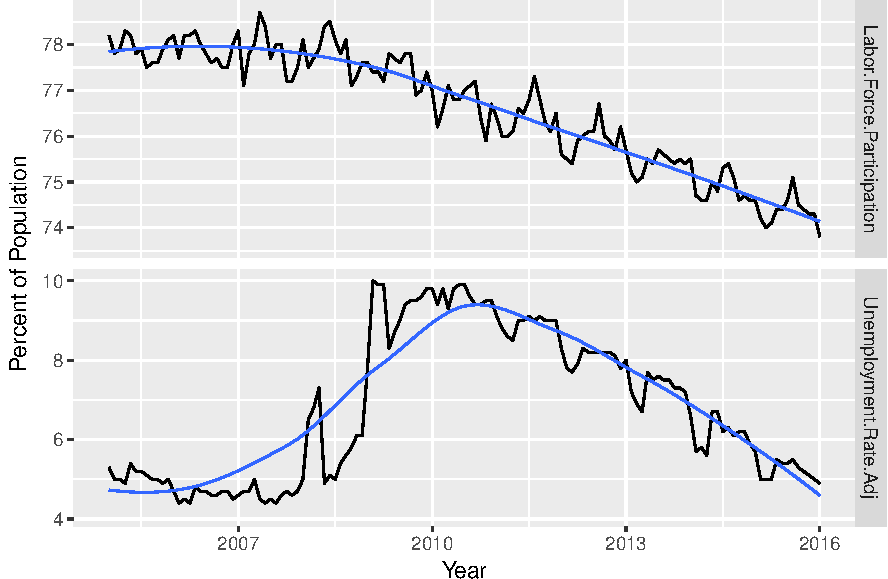
\includegraphics{elliott-econometric-personnel-retention-18_files/figure-latex/lfpr-unemployment-1} 

}

\caption{Participation and Unemployment}\label{fig:lfpr-unemployment}
\end{figure}

It is assumed that the skillsets of our target population (non-rated
line officers) are most transferrable to those jobs covered by nonfarm
payrolls. Nonfarm is a category that excludes proprietors, private
household employees, unincorporated self-employment, unpaid volunteers,
and farm employees \cite{fred-nonfarm-2017}. Job quits are generally
voluntary separations and may reflect workers' willingness to leave; it
may be that the a higher propensity to volutarily leave a job translates
to a positive outlook on obtaining another.

The labor market momentum index compares current labor market conditions
to historical averages. A negative value indicates conditions below the
long-term average, and a positive value indicates favorable conditions.
The CPI examines the weighted average price of a basket of consumer
goods and services; it is used to estimate the cost of living. There is
some uncertainty involving employment in separation from the military,
so cost of living information may be especially important to that
decision as the military is excluded from CPI statistics.

By including these variables in a regression model and estimating their
effects, this thesis is attempting to capture military members'
perceptions of economic health and job prospects, and use that
information as a means to forecast attrition.

\hypertarget{cleaning-and-preparation}{%
\subsection{Cleaning and Preparation}\label{cleaning-and-preparation}}

Perfect data is rarely found or received outside of the classroom, and
such is the case here. Before exploration and modeling, several steps
are taken to produce a useable data set.

The personnel data is first converted from long to wide format. This
procedure generates missing values, and they need to be dealt with
appropriately. Missing values can result from several underlying issues:
data storage corruption, entry errors, miscommunication between
software, etc. Luckily, none of those apply here. Since the attrition
data is a monthly count of people exiting USAF service, the intuition is
that these missing values simply represent a lack of an observation
(i.e.~zero separations). This is confirmed by the data's provider, and
so all missing values are replaced with zero. Initially, observation
dates are stored as the number of days since 1 Jan 1960 (the standard
for SAS). This is transformed into YYYY-MM-DD, in order to merge with
the economic data. Several columns are added, each the total separations
for a specific subset of the officer corps: rated, non-rated line,
non-line, etc. These sums will be the responses used for modeling.

The economic data does not require much treatment, as it comes from a
professionally managed database. One of the indicators, real GDP per
capita, occurs in quarterly intervals - the rest are monthly. In order
to combine, the observation for a quarter is carried through the quarter
(e.g.~the observation for Q1 2006 is applied to January, Febuary, and
March 2006). Then, variables are renamed for clarity. Finally, economic
data are merged with the personnel through an inner join, preserving
only those observations in common.

\hypertarget{model-selection}{%
\section{Model Selection}\label{model-selection}}

\hypertarget{initial-exploration}{%
\subsection{Initial Exploration}\label{initial-exploration}}

Before throwing around modeling techniques, the data is visually
inspected. Plotting one response, total separations over all career
fields, in Figure \ref{fig:response-plot} shows significant spikes
during 2005, '06, '07, and '14. We know that during these periods,
special spearation incentive programs were introduced in order to
artificially downsize the air force. The effects of these periods merit
investigation later on, as they could negatively affect model
performance.

\begin{figure}[H]

{\centering 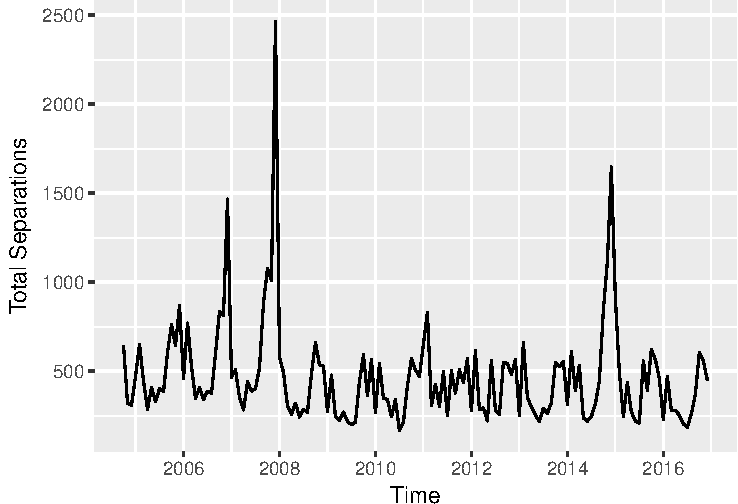
\includegraphics{elliott-econometric-personnel-retention-18_files/figure-latex/response-plot-1} 

}

\caption{Monthly Officer Separations}\label{fig:response-plot}
\end{figure}

No seasonality is immediately obvious in Figure \ref{fig:response-plot}.
However, if each year is plotted separately, a clearer picture emerges.
First, Figure \ref{fig:response-season-plot} shows that the extreme
points noticed noticed above seem to be relegated to the
November-December time frame. Second, it is easier to witness the
seasonality: bowing across the year, with higher counts at the beginning
and end.

\begin{figure}[H]

{\centering 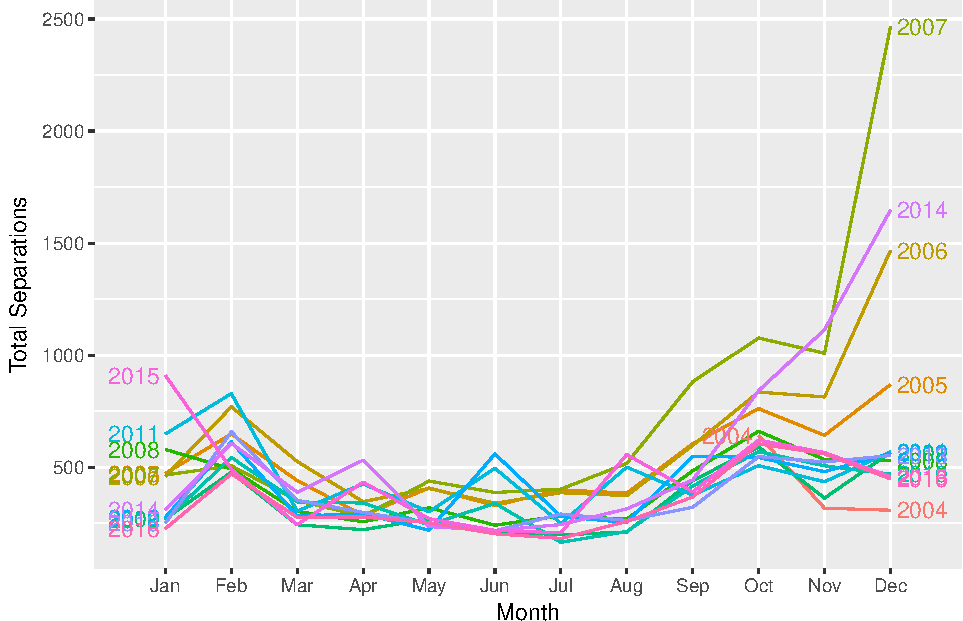
\includegraphics{elliott-econometric-personnel-retention-18_files/figure-latex/response-season-plot-1} 

}

\caption{Seasonal Plot: Total Separations}\label{fig:response-season-plot}
\end{figure}

Considering these plots, we expect that a seasonal model performs best
and that we will have to perform some alteration to accomodate the
outiers. To confirm, we fit naive models to the data and examine to
results. Beyond revealing seasonlity and outlier effects, fitting naive
models serves to establish a baseline to compare later models against.
Naive models are as simplistic as possible, so if later models perform
worse or only marginally better, it implies they are not capturing much
information.

Figure \ref{fig:n-sn-forecast} gives evidence to the negative effects of
outliers, notice the large confidence intervals surrounding the naive
forecast and the 2014 spike carried through in the seasonal forecast.

\begin{figure}[H]

{\centering 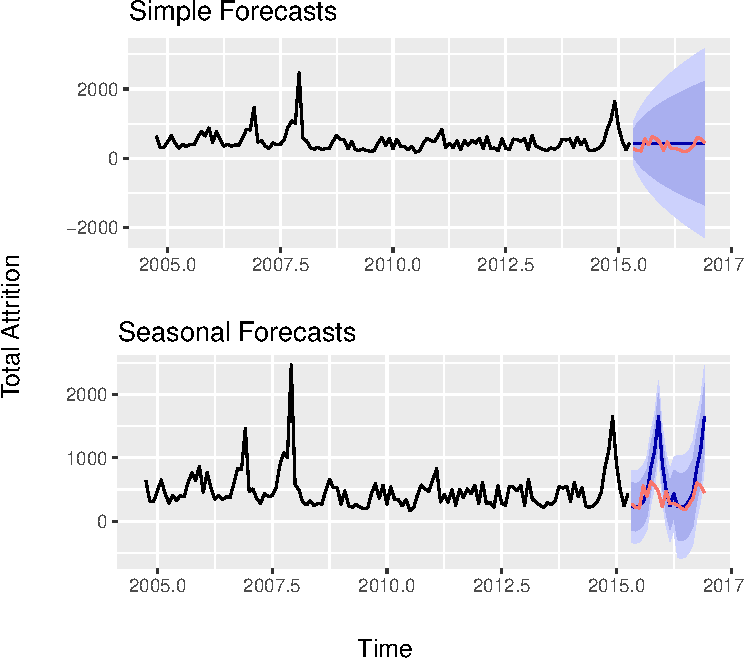
\includegraphics{elliott-econometric-personnel-retention-18_files/figure-latex/n-sn-forecast-1} 

}

\caption{Simple and Seasonal Naive Forecasts}\label{fig:n-sn-forecast}
\end{figure}

Tables \ref{fig:n-err} and \ref{fig:sn-err} show different error metrics
for each of the two models. By mean square error (MSE), the seasonal
model generally fits the training data better, possibily indicating
presence of seasonality effects. However, there is a large disparity
between validation MSEs, possibly caused by the major spike in 2014 -
reaffirming the earlier intuition about outlier effects.

\begin{table}

\caption{\label{tab:n-err}Naive Results}
\centering
\begin{tabular}[t]{l|r|r|r|r|r|r}
\hline
  & ME & RMSE & MAE & MPE & MAPE & MASE\\
\hline
Training set & -1.650794 & 312.5230 & 195.9841 & -12.53034 & 42.09254 & 1.2607358\\
\hline
Test set & -62.600000 & 160.6421 & 144.3000 & -37.26534 & 51.56901 & 0.9282598\\
\hline
\end{tabular}
\end{table}\begin{table}

\caption{\label{tab:sn-err}Seasonal Naive Results}
\centering
\begin{tabular}[t]{l|r|r|r|r|r|r}
\hline
  & ME & RMSE & MAE & MPE & MAPE & MASE\\
\hline
Training set & 16.49565 & 291.7907 & 155.4522 & -7.373817 & 30.45221 & 1.000000\\
\hline
Test set & -238.85000 & 454.2881 & 271.4500 & -59.852083 & 67.31547 & 1.746196\\
\hline
\end{tabular}
\end{table}

It is known that during years 2005, '06, '07, and '14 special separation
programs were implemented. Given the effect those years appear to have
on modeling, they ought to be dealt with before continuing. Before
deciding how, the explicit points in question need to be identified. To
help, refer back to Figure \ref{fig:response-season-plot}. We note above
that the spikes generally occur in November and December. However, the
observations from 2005 are close enough to those from other years that
they may have resulted naturally. We do not want to remove too much
information from the data set, only that which is misleading. So,
November and December observations from 2006, '07, and '14 are selected
for replacement.

Given the seasonality in the data set, the replaced values should stem
from matching observations in previous years, as opposed to previous
observations within the same year. The outliers are replaced with the
arithmetic mean of all years not being replaced (e.g.~November 2006,
'07, '14 is replaced with the mean separations in November for all other
years).

Replotting the repsonse in Figure \ref{fig:response-plot-2} shows a much
better behaved data set. The data look fairly stationary, setting the
stage for more forecasting complex models.

\begin{figure}[H]

{\centering 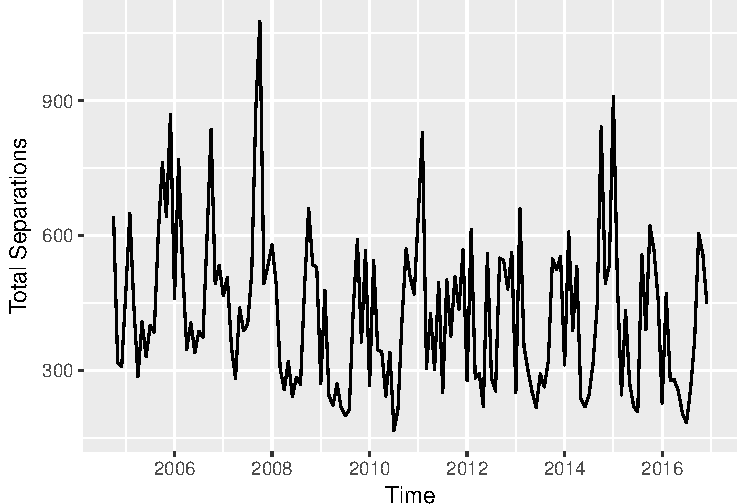
\includegraphics{elliott-econometric-personnel-retention-18_files/figure-latex/response-plot-2-1} 

}

\caption{Separations - Outliers Removed}\label{fig:response-plot-2}
\end{figure}

With the outliers replaced, seasonal effects are much more apparent as
well (see Figure \ref{fig:response-season-plot-2} below), further
enforcing the need for a seasonal model.

\begin{figure}[H]

{\centering 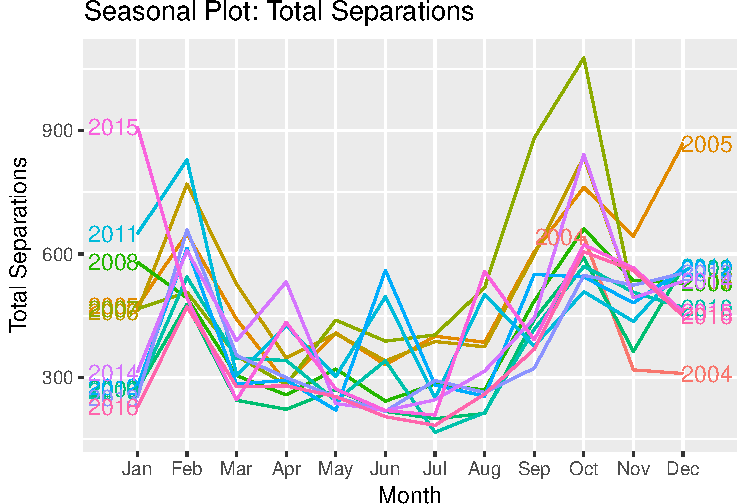
\includegraphics{elliott-econometric-personnel-retention-18_files/figure-latex/response-season-plot-2-1} 

}

\caption{Seasonal Plot: Outliers Removed}\label{fig:response-season-plot-2}
\end{figure}

The purpose of imputing those values was to help produce better models.
That can be assessed by retraining the naive models and comparing
against previous results.

Table \ref{fig:season-rmse-compare} below compares the seasonal naive
RMSEs before and after imputating the identified outliers. The results
indicate that removing and replacing the extreme values for November and
December improved the model's ability to capture information. This is
further reflected by the forecast (shown in blue) in Figure
\ref{fig:sn-forecast-2}, which follows the validation data (shown in
orange) more closely than those in Figure \ref{fig:n-sn-forecast}.
Overall, these results imply that imputation of the selected
observations is a worthwhile endeavor.

\begin{table}

\caption{\label{tab:season-rmse-compare}Seasonal Naive RMSE Comparison}
\centering
\begin{tabular}[t]{l|r|r}
\hline
  & Raw Data & Imputed Data\\
\hline
Training & 291.7907 & 161.2624\\
\hline
Validation & 454.2881 & 186.5842\\
\hline
\end{tabular}
\end{table}

\begin{figure}[H]

{\centering 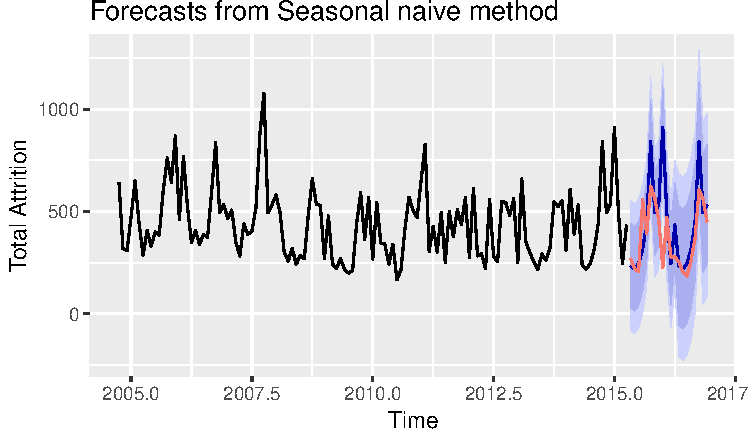
\includegraphics{elliott-econometric-personnel-retention-18_files/figure-latex/sn-forecast-2-1} 

}

\caption{Seasonal Naive Forecast After Imputation}\label{fig:sn-forecast-2}
\end{figure}

Though an important step in the modeling process, these naive models are
not the end goal. Rather, they help identify initial road bumps in the
modeling process and create a baseline against which to compare other,
more sophisticated models.

\hypertarget{model-specification}{%
\subsection{Model Specification}\label{model-specification}}

One major shortfall of the naive model is the inability to include
exogenous information, and this is is case for many forecasting methods
(ARIMA, Decomposition, Exponential Smoothing, etc). However, these
methods do allow the inclusion of autoregressive information, which
normal regression techniques do not.

The solution, then, is to combine efforts with dynamic regression.
Dynamic regression is just a multivariate regression model with an ARIMA
model on the errors. The regression piece allows independent variables
to be used in predicting a response, and the ARIMA portion helps capture
and account for autoregressive information which often exists in
time-series data (thereby helping preserve the assumption of independent
errors). The general formulation of a dynamic regression model (with
ARIMA(1,1,1), for example) errors is:

\[ y_t = \beta_0 + \beta_1x_{1,t} + ... + \beta_kx_{k,t} + n_t\] where,

\[ (1-\phi_1B)(1-B)n_t = (1+\theta_1B)e_t \] and \(e_t\) is white noise.

Before fitting the dynamic regression model, several steps must be taken
to ensure other key assumptions are not violated. First

\newpage

\hypertarget{conclusions}{%
\chapter{Conclusions}\label{conclusions}}

This is the final chapter of your thesis.
\newpage
%==================================================================
%    		Bibliography              
%==================================================================
\addcontentsline{toc}{chapter}{\bfseries Bibliography}
\singlespace
\bibliography{references/my_bib}
%==================================================================
%    		Vita              
%==================================================================
    \newpage
    \addcontentsline{toc}{chapter}{\bfseries Vita}
    \begin{center}
	\Large\bfseries Vita
    \end{center}
    \vspace{2em}
    \doublespacing
    The vita.
    \newpage
%==================================================================
%    		SF298             
%==================================================================
\pagestyle{empty}
\newgeometry{vmargin=0.2in,hmargin=0.4in}
\singlespace
\everyTextField{
            \BC{0.98 0.92 0.73} \BG{1 1 1}
            \textColor{0 0 0}   \textFont{helv}     \textSize{10} 
            \Q{0}               \W{0}
            } 
\everySigField{
            \BC{0.98 0.92 0.73} \BG{0.98 0.92 0.73}
            \textColor{0 0 0}   \textFont{helv}     \textSize{10} 
            \Q{1}               \W{0}
            } 
\newdimen\rhI       \rhI=0.04\textheight
\newdimen\rhII      \rhII=0.08\textheight
\newdimen\rhIII     \rhIII=0.04\textheight
\newdimen\rhIV      \rhIV=0.12\textheight
\newdimen\rhV       \rhV=\rhIV
\newdimen\rhVI      \rhVI=.09\textheight
\newdimen\rhVII     \rhVII=0.09\textheight
\newdimen\rhVIII    \rhVIII=0.07\textheight
\newdimen\rhIX      \rhIX=0.05\textheight
\newdimen\rhX       \rhX=0.16\textheight
\newdimen\rhXI      \rhXI=0.04\textheight
\newdimen\rhXII     \rhXII=0.01\textheight
\begin{myfont}
\noindent\resizebox{\textwidth}{!}{%
\begin{tabular}{|l|}
\hline
%==================================================================
%    		Page 1 - Row 1              
%==================================================================
\parbox[][\rhI][c]{0.70\textwidth}{
\centering
\textbf{REPORT DOCUMENTATION PAGE}
} \vrule\hspace{1pt}

\parbox[][\rhI][c]{0.30\textwidth}{
\centering
\small Form Approved\\[-1pt]
\small OMB No. 0704-0188
}\\\hline
%==================================================================
%    		Page 1 - Row 2
%==================================================================
\parbox[][\rhII][t]{\textwidth}{
\vspace{2pt}
\begin{spacing}{0.7}
\footnotesize\raggedright The public reporting burden for this collection of information is estimated to average 1 hour per response, including the time for reviewing instructions, searching existing data sources, gathering and maintaining the data needed, and completing and reviewing the collection of information. Send comments regarding this burden estimate or any other aspect of this collection of information, including suggestions for reducing the burden, to Department of Defense, Washington Headquarters Services, Directorate for Information Operations and Reports (0704-0188), 1215 Jefferson Davis Highway, Suite 1204, Arlington, VA 22202-4302. Respondents should be aware that notwithstanding any other provision of law, no person shall be subject to any penalty for failing to comply with a collection of information if it does not display a currently valid OMB control number.\linebreak \textbf{PLEASE DO NOT RETURN YOUR FORM TO THE ABOVE ADDRESS.}
\end{spacing}
}\\\hline
%==================================================================
%    		Page 1 - Row 3
%==================================================================
\parbox[][\rhIII][c]{.25\textwidth}{
\vspace{0pt}
\small 1. REPORT DATE (DD-MM-YYYY)\\[2pt]
\textField[\TU{ }\V{30-01-2018}]{sf1}{.24\textwidth}{0.4cm}
}\vrule\hspace{1pt}

\parbox[][\rhIII][c]{.45\textwidth}{
\vspace{1pt}
\small 2. REPORT TYPE\\[2pt]
\textField[\TU{ }\V{Thesis}]{sf2}{.44\textwidth}{0.4cm}
}\vrule\hspace{1pt}

\parbox[][\rhIII][c]{0.30\textwidth}{
\vspace{0pt}
\small 3. DATES COVERED (From - To)\\[2pt]
\textField[\TU{ }\V{}]{sf3}{.29\textwidth}{0.4cm}
}\\\hline
\end{tabular}}\\
%==================================================================
%    		Page 1 - Row 4
%==================================================================
\noindent\resizebox{\textwidth}{!}{%
\begin{tabular}{|l|l|}
\multirow{3}*{
\parbox[][\rhIV][c]{0.65\textwidth}{
\vspace{-25pt}
\small 4. TITLE AND SUBTITLE\\[2pt]
\textField[\Ff{\FfMultiline}\textSize{11}\TU{ }\V{\uppercase{Air Force Officer Attrition: An Econometric Analysis}}]{sf4}{.64\textwidth}{2.4cm}
}} &

\parbox[][0.33\rhIV][c]{0.35\textwidth}{
\small 5a. CONTRACT NUMBER\\[2pt]
\textField[\TU{ }\V{DACA99-99-C-9999}]{sf5a}{.34\textwidth}{0.4cm}
}\bigstrut\\\cline{2-2}
&

\parbox[][0.33\rhIV][c]{0.35\textwidth}{
\small 5b. GRANT NUMBER\\[2pt]
\textField[\TU{ }\V{}]{sf5b}{.34\textwidth}{0.4cm}
}\bigstrut\\\cline{2-2}
&

\parbox[][0.33\rhIV][c]{0.35\textwidth}{
\small 5c. PROGRAM ELEMENT NUMBER\\[2pt]
\textField[\TU{ }\V{}]{sf5c}{.34\textwidth}{0.4cm}
}\bigstrut\\\hline
\end{tabular}}
%==================================================================
%    		Page 1 - Row 5
%==================================================================
\noindent\resizebox{\textwidth}{!}{%
\begin{tabular}{|l|l|}
\multirow{3}*{
\parbox[][\rhV][c]{0.65\textwidth}{
\vspace{-25pt}
\small 6. AUTHOR(S)\\[2pt]
\textField[\textSize{11}\Ff{\FfMultiline}\TU{ }\V{Elliott, Jacob, T, 1st Lt, USAF}]{sf6}{.64\textwidth}{2.4cm}
}} & 

\parbox[][0.33\rhIV][c]{0.35\textwidth}{
\small 5d. PROJECT NUMBER\\[2pt]
\textField[\TU{ }\V{}]{sf5d}{.34\textwidth}{0.4cm}
}\bigstrut\\\cline{2-2}
&

\parbox[][0.33\rhIV][c]{0.35\textwidth}{
\small 5e. TASK NUMBER\\[2pt]
\textField[\TU{ }\V{}]{sf5e}{.34\textwidth}{0.4cm}
}\bigstrut\\\cline{2-2}
&

\parbox[][0.33\rhIV][c]{0.35\textwidth}{
\small 5f. WORK UNIT NUMBER\\[2pt]
\textField[\TU{ }\V{}]{sf5f}{.34\textwidth}{0.4cm}
}\bigstrut\\\hline
\end{tabular}}
%==================================================================
%    		Page 1 - Row 6
%==================================================================
\noindent\resizebox{\textwidth}{!}{%
\begin{tabular}{|l|}
\parbox[][\rhVI][c]{0.70\textwidth}{
\small 7. PERFORMING ORGANIZATION NAMES(S) AND ADDRESS(ES)\\[2pt]
\textField[\Ff{\FfMultiline}\TU{ }\V{
Air Force Institute of Technology\n
Graduate School of Engineering and Management (AFIT/Department of Operational Sciences)\n
2950 Hobson Way, Building 640\n
WPAFB OH 45433-7301}]{sf7}{.69\textwidth}{1.8cm}
} \vrule\hspace{1pt}

\parbox[][\rhVI][c]{0.30\textwidth}{\vspace{-10pt}
\small \begin{spacing}{0.75}\begin{tabbing}8. \=PERFORMING ORGANIZATION \\ \>REPORT NUMBER\end{tabbing}\end{spacing}\vspace{10pt}
\textField[\TU{ }\V{AFIT-ENS-MS-18-M-118}]{sf5f}{.29\textwidth}{.5cm}
}\\\hline
\end{tabular}}
%==================================================================
%    		Page 1 - Row 7
%==================================================================
\noindent\resizebox{\textwidth}{!}{%
\begin{tabular}{|l|l|}
\multirow{2}*{
\parbox[][\rhVII][c]{0.70\textwidth}{\vspace{-20pt}
\small 9. SPONSORING/MONITORING AGENCY NAME(S) AND ADDRESS(ES)\\[2pt]
\textField[\Ff{\FfMultiline}\TU{ }\V{\n
\n
\n
\n
}]{sf9}{.69\textwidth}{1.8cm}
}} & 

\parbox[][0.425\rhVII][c]{0.30\textwidth}{
\small 10. SPONSOR/MONITOR ACRONYM(S)\\[2pt]
\textField[\TU{ }\V{}]{sf10}{.29\textwidth}{0.4cm}
}\bigstrut\\\cline{2-2}
&

\parbox[][0.575\rhVII][c]{0.30\textwidth}{\vspace{-10pt}
\small \begin{spacing}{0.75}\begin{tabbing}11. \=SPONSOR/MONITOR REPORT \\\> NUMBER(S)\end{tabbing}\end{spacing}\vspace{-10pt}
\textField[\TU{ }\V{}]{sf11}{.29\textwidth}{0.4cm}
}\bigstrut\\\hline
\end{tabular}}
%==================================================================
%    		Page 1 - Row 8
%==================================================================
 \noindent\resizebox{\textwidth}{!}{%
 \begin{tabular}{|l|}
\parbox[][\rhVIII][c]{\textwidth}{
\small 12. DISTRIBUTION/AVAILABILITY STATEMENT\\[2pt]
\textField[\Ff{\FfMultiline}\TU{ }\V{}]{sf12}{\textwidth}{1.2cm}
}\bigstrut\\\hline

\parbox[][\rhIX][c]{\textwidth}{
\small 13. SUPPLEMENTARY NOTES\\[2pt]
\textField[\Ff{\FfMultiline}\TU{ }\V{ }]{sf13}{\textwidth}{.8cm}
}\bigstrut\\\hline

\parbox[][\rhX][c]{\textwidth}{
\small 14. ABSTRACT\\[2pt]
\textField[\Ff{\FfMultiline}\TU{ }\V{The abstract of the thesis.}]{sf14}{\textwidth}{3.8cm}
}\bigstrut\\\hline

\parbox[][\rhXI][c]{\textwidth}{
\small 15. SUBJECT TERMS\\[2pt]
\textField[\TU{ }\V{}]{sf15}{\textwidth}{0.4cm}
}\bigstrut\\\hline
 \end{tabular}}
%==================================================================
%    		Page 1 - Row 8
%==================================================================
\noindent\resizebox{\textwidth}{!}{

\begin{tabular}{|l|l|l|l|l|l|}
\multicolumn{3}{|l|}{\parbox[][0.2\rhXII][c]{0.30\textwidth}{\small 16. SECURITY CLASSIFICATION OF:}} &
\multirow{6}{0.15\textwidth}{\parbox[][\rhXII][t]{0.15\textwidth}{\vspace{-35pt}
\small \begin{spacing}{0.75}\begin{tabbing}17. \=LIMITATION OF \\\> ABSTRACT\end{tabbing}\end{spacing}
\vspace{4pt}
\textField[\Q{1}\TU{ }\V{}]{sf17}{.15\textwidth}{0.4cm}}} &

\multirow{6}{0.09\textwidth}{\parbox[][\rhXII][t]{0.09\textwidth}{\vspace{-35pt}
\small \begin{spacing}{0.75}\begin{tabbing} 18. \=NUMBER \\\>OF\\\> PAGES \end{tabbing}\end{spacing}
\vspace{-5pt}
\textField[\Q{1}\TU{ }\V{30}]{sf18}{.09\textwidth}{0.4cm}}} &

\multirow{3}{0.4\textwidth}{\parbox[][0.5\rhXII][t]{0.4\textwidth}{\vspace{-12pt}
\small 19a. NAME OF RESPONSIBLE PERSON\\[4pt]
\textField[\textSize{11}\TU{ }\V{}]{sf19a}{.40\textwidth}{0.4cm}}}\\\cline{1-3}

\multirow{5}{0.12\textwidth}{\parbox[][0.8\rhXII][t]{0.12\textwidth}{\vspace{-20pt}
\small a. REPORT\\[15pt]
\textField[\Q{1}\TU{ }\V{}]{sf16a}{.12\textwidth}{0.4cm}}} & 

\multirow{5}{0.12\textwidth}{\parbox[][0.8\rhXII][t]{0.12\textwidth}{\vspace{-20pt}
\small b. ABSTRACT\\[15pt]
\textField[\Q{1}\TU{ }\V{}]{sf16b}{.12\textwidth}{0.4cm}}} & 

\multirow{5}{0.12\textwidth}{\parbox[][0.8\rhXII][t]{0.12\textwidth}{\vspace{-20pt}
\small c. THIS PAGE\\[15pt]
\textField[\Q{1}\TU{ }\V{}]{sf16c}{.12\textwidth}{0.4cm}}} & & & \\ 
& & & & & \\ \cline{6-6}
& & & & & \multirow{3}{0.4\textwidth}{\parbox[][0.5\rhXII][t]{0.4\textwidth}{\vspace{-10pt}
\small 19b. PHONE NUMBER (Include area code)\\[4pt]
\textField[\textSize{10}\TU{ }\V{937-255-3636 x7469advisor@afit.edu}]{sf19b}{.4\textwidth}{0.4cm}}} \\
& & & & & \\
& & & & & \\ \cline{1-6}
\end{tabular}}
\end{myfont}
\end{document}
